\chapter{Specifikacija programske potpore}
		
	\section{Funkcionalni zahtjevi}
			
			\noindent \textbf{Dionici:}
			
			\begin{packed_enum}
				
				\item Igrači
				\begin{packed_enum}
				    \item Igrač početnik
				    \item Napredni igrač
				\end{packed_enum}
				\item Kartograf				
				\item Administrator
				\item Razvojni tim
				
			\end{packed_enum}
			
			\noindent \textbf{Aktori i njihovi funkcionalni zahtjevi:}
			
			
			\begin{packed_enum}
				\item  \underbar{Neregistrirani/neprijavljeni korisnik (inicijator) može:}
				
				\begin{packed_enum}
					
					\item vidjeti stranicu dobrodošlice na kojoj se nalaze upute za korištenje aplikacije
					\item pregledati dostupne kartice na karti
					\item vidjeti globalnu statistiku odigranih borbi i sakupljenih lokacija te poredak svih igrača
					\item se registrirati u sustav, stvoriti novi korisnički račun za koji su mu potrebni korisničko ime, fotografija, lozinka i e-mail adresa
					
				\end{packed_enum}
			
				\item  \underbar{Igrač početnik (inicijator) može:}
				
				\begin{packed_enum}
					
					\item sakupljati lokacije, tj. kartice
					\item vidjeti popis ostalih aktivnih igrača koji se nalaze unutar 50 km i s njima ući u borbu
					
					\begin{packed_enum}
					    
					    \item odabir skupa karata s kojima će se boriti
					    
					\end{packed_enum}
					
					\item pristupiti pregledu profila igrača
					
					\begin{packed_enum}
					    
					    \item prikaz svih karata koje je igrač skupio
					    \item prikaz ranga na globalnoj ljestvici
					    \item prikaz statistike vezane uz zadnjih 10 borbi s drugim igračima
					    
					\end{packed_enum}
					
				\end{packed_enum}
				
			\item  \underbar{Napredni igrač (inicijator) može:}
				
				\begin{packed_enum}
					
					\item sakupljati lokacije, tj. kartice
					\item vidjeti popis ostalih aktivnih igrača koji se nalaze unutar 50 km i s njima ući u borbu
					
					\begin{packed_enum}
					    
					    \item odabir skupa karata s kojima će se boriti
					    
					\end{packed_enum}
					
					\item pristupiti pregledu profila igrača
					
					\begin{packed_enum}
					    
					    \item prikaz svih karata koje je igrač skupio
					    \item prikaz ranga na globalnoj ljestvici
					    \item prikaz statistike vezane uz zadnjih 10 borbi s drugim igračima
					    
					\end{packed_enum}
					
					\item prijaviti novu lokaciju (s potrebnim podacima) u čijoj se neposrednoj blizini nalazi
					
				\end{packed_enum}
				
			\item \underbar{Kartograf (inicijator) može:}
			
			    \begin{packed_enum}
			    
			        \item se registrirati za što su mu potrebni IBAN račun za uplatu i fotografija osobne iskaznice
			        \item nadopuniti bazu podatka s lokacijama koje su igrači prijavili
			        \item vidjeti prijave na karti
			        
			        \begin{packed_enum}
			            
			            \item odbijanje, potvrđivanje i uređivanje prijave
			            \item oznaka za potrebnu potvrdu s terena
			          
			        \end{packed_enum}
			        
			        \item označiti koje će prijave osobno provjeriti
			        
			    \end{packed_enum}
			    
		    \item \underbar{Administrator (inicijator) može:}
		    
		        \begin{packed_enum}
		            
		            \item vidjeti i uređivati popis svih registriranih korisnika i njihovih osobnih podataka
		            \item uređivati postojeće lokacije u igri
		            \item dodijeliti igračima privremeno isključenje iz igre
		            
		        \end{packed_enum}
		        
	        \item \underbar{Baza podataka (sudionik):}
		    
		        \begin{packed_enum}
		            
		            \item pohranjuje sve podatke o korisnicima i njihovim ovlastima
		            \item pohranjuje sve podatke o lokacijama
		            \item pohranjuje sve  podatke o provedenim borbama i izazovima
		            
		        \end{packed_enum}
		        
			\end{packed_enum}
			
			\eject 
			
			
				
			\subsection{Obrasci uporabe}
				
				
					\noindent \underbar{\textbf{UC1 - Registracija kao igrač}}
					\begin{packed_item}
	
						\item \textbf{Glavni sudionik: }Gost
						\item  \textbf{Cilj:} Stvoriti korisnički račun za pristup sustavu
						\item  \textbf{Sudionici:} Baza podataka
						\item  \textbf{Preduvjet:} -
						\item  \textbf{Opis osnovnog tijeka:}
						
						\item[] \begin{packed_enum}
	
							\item Gost odabire opciju za registraciju igrača
							\item Gost unosi potrebne korisničke podatke
							\item Gost dobiva e-mail kojim potvrđuje svoj račun

						\end{packed_enum}
						
						\item  \textbf{Opis mogućih odstupanja:}
						
						\item[] \begin{packed_item}
	
							\item[2.a] Odabir već zauzetog korisničkog imena i/ili e-maila, unos korisničkog podatka u nedozvoljenom formatu ili pružanje neispravnog e-maila
							\item[] \begin{packed_enum}
								
								\item Sustav obavještava korisnika o neuspjelom upisu i vraća ga na stranicu za registraciju
								\item Korisnik mijenja potrebne podatke te završava unos ili odustaje od registracije
								
							\end{packed_enum}
							
						\end{packed_item}
					\end{packed_item}
					
					\noindent \underbar{\textbf{UC2 - Registracija kao kartograf}}
					\begin{packed_item}
	
						\item \textbf{Glavni sudionik: }Gost
						\item  \textbf{Cilj:} Stvoriti korisnički račun za pristup sustavu
						\item  \textbf{Sudionici:} Baza podataka
						\item  \textbf{Preduvjet:} -
						\item  \textbf{Opis osnovnog tijeka:}
						
						\item[] \begin{packed_enum}
	
							\item Korisnik odabire opciju za registraciju kartografa
							\item Korisnik unosi potrebne korisničke podatke
							\item Korisnik dobiva e-amil kojim potvrđuje svoju prijavu
							\item Korisnika administratori potvrđuju kao kartografa

						\end{packed_enum}
						
						\item  \textbf{Opis mogućih odstupanja:}
						
						\item[] \begin{packed_item}
	
							\item[2.a] Odabir već zauzetog korisničkog imena i/ili e-maila, unos korisničkog podatka u nedozvoljenom formatu, pružanje neispravnog e-maila ili unos neispravnog IBAN-a
							\item[] \begin{packed_enum}
								
								\item Sustav obavještava korisnika o neuspjelom upisu i vraća ga na stranicu za registraciju
								\item Korisnik mijenja potrebne podatke te završava unos ili odustaje od registracije
								
							\end{packed_enum}
							
						\end{packed_item}
					\end{packed_item}
				
				    \noindent \underbar{\textbf{UC3 - Prijava u sustav}}
					\begin{packed_item}
	
						\item \textbf{Glavni sudionik:} Korisnik
						\item  \textbf{Cilj:} Dobiti pristup korisničkom sučelju
						\item  \textbf{Sudionici:} Baza podataka
						\item  \textbf{Preduvjet:} Registracija
						\item  \textbf{Opis osnovnog tijeka:}
						
						\item[] \begin{packed_enum}
	
							\item Unos korisničkog imena i lozinke
							\item Potvrda o ispravnosti unesenih podataka
							\item Pristup korisničkim funkcijama

						\end{packed_enum}
						
						\item  \textbf{Opis mogućih odstupanja:}
						
						\item[] \begin{packed_item}
	
							\item[2.a] Neispravno korisničko ime/e-mail/lozinka
							\item[] \begin{packed_enum}
								
								\item Sustav obavještava korisnika o neuspjelom upisu i vraća ga na stranicu za registraciju
								
							\end{packed_enum}
							
						\end{packed_item}
					\end{packed_item}
					
					\noindent \underbar{\textbf{UC4 - Pregled osobnih podataka}}
					\begin{packed_item}
	
						\item \textbf{Glavni sudionik: }Korisnik
						\item  \textbf{Cilj:} Pregledati osobne podatke i statistike
						\item  \textbf{Sudionici:} Baza podataka
						\item  \textbf{Preduvjet:} Korisnik je prijavljen
						\item  \textbf{Opis osnovnog tijeka:}
						
						\item[] \begin{packed_enum}
	
							\item Korisnik odabire opciju \textit{My Profile}
							\item Aplikacija prikazuje osobne podatke korisnika i njegovu statistiku

						\end{packed_enum}
						
					\end{packed_item}
					
					\noindent \underbar{\textbf{UC5 - Pregled profila drugih igrača}}
					\begin{packed_item}
	
						\item \textbf{Glavni sudionik: }Igrač
						\item  \textbf{Cilj:} Pregledati profil drugog igrača
						\item  \textbf{Sudionici:} Baza podataka
						\item  \textbf{Preduvjet:} Igrač je prijavljen
						\item  \textbf{Opis osnovnog tijeka:}
						
						\item[] \begin{packed_enum}
							\item Korisnik se nalazi na bilo kojoj stranici koja mu prikazuje korisničko ime drugog igrača
							\item Korisnik klikom na korisničko ime igrača zahtijeva pregled njegovog profila
							\item Korisniku se prikazuje javni profil odabranog korisnika
						\end{packed_enum}
					\end{packed_item}
					
					\noindent \underbar{\textbf{UC6 - Uređivanje vlastitih podataka}}
					\begin{packed_item}
	
						\item \textbf{Glavni sudionik: }Korisnik
						\item  \textbf{Cilj:} Urediti osobne podatke
						\item  \textbf{Sudionici:} Baza podataka
						\item  \textbf{Preduvjet:} Korisnik je prijavljen
						\item  \textbf{Opis osnovnog tijeka:}
						
						\item[] \begin{packed_enum}
	
							\item Korisnik odabire opciju za promjenu podataka
							\item Korisnik mijenja svoje osobne podatke
							\item Korisnik sprema promjene
							\item Baza podataka se ažurira

						\end{packed_enum}
						
						\item  \textbf{Opis mogućih odstupanja:}
						
						\item[] \begin{packed_item}
	
							\item[2.a] Korisnik promijeni svoje osobne podatke, ali ne odabere opciju \textit{Save changes}
							\item[] \begin{packed_enum}
								
								\item Sustav obavještava korisnika da nije spremio podatke prije izlaska iz prozora
								
							\end{packed_enum}
							
						\end{packed_item}
					\end{packed_item}
					
					\noindent \underbar{\textbf{UC7 - Brisanje korisničkog računa}}
					\begin{packed_item}
	
						\item \textbf{Glavni sudionik: }Korisnik
						\item  \textbf{Cilj:} Izbrisati svoj račun
						\item  \textbf{Sudionici:} Baza podataka
						\item  \textbf{Preduvjet:} Korisnik je prijavljen
						\item  \textbf{Opis osnovnog tijeka:}
						
						\item[] \begin{packed_enum}
	
							\item Korisnik pregledava osobne podatke
							\item Otvara se stranica s osobnim podacima korisnika
							\item Korisnik briše račun
							\item Korisnički račun se izbriše iz baze podataka
							\item Otvara se stranica za registraciju

						\end{packed_enum}
				
					\end{packed_item}
					
					\noindent \underbar{\textbf{UC8 - Skupljanje kartice}}
					\begin{packed_item}
	
						\item \textbf{Glavni sudionik: }Igrač
						\item  \textbf{Cilj:} Pokupiti karticu
						\item  \textbf{Sudionici:} Baza podataka
						\item  \textbf{Preduvjet:} Korisnik je prijavljen i nalazi se u neposrednoj blizini lokacije na kojoj je kartica
						\item  \textbf{Opis osnovnog tijeka:}
						
						\item[] \begin{packed_enum}
	
							\item Korisnik odabire karticu na karti
							\item Korisnik odabire opciju \textit{Collect}
							\item Kartica se nalazi na stranici \textit{My Profile -$>$ Inventory} 

						\end{packed_enum}
						
						\item  \textbf{Opis mogućih odstupanja:}
						
						\item[] \begin{packed_item}
	
							\item[2.a] Odabir kartice koju nije moguće pokupiti s korisnikove trenutne lokacije
							\item[] \begin{packed_enum}
								
								\item Sustav obavještava korisnika o neuspjelom sakupljanju kartice
								
							\end{packed_enum}
							
						\end{packed_item}
					\end{packed_item}
					
					\noindent \underbar{\textbf{UC9 - Pregled globalne statistike}}
					\begin{packed_item}
					
						\item \textbf{Glavni sudionik: }Korisnik
						\item  \textbf{Cilj:} Pregledati globalnu statistiku
						\item  \textbf{Sudionici:} Baza podataka
						\item  \textbf{Preduvjet:} Korisnik je prijavljen
						\item  \textbf{Opis osnovnog tijeka:}
						
						\item[] \begin{packed_enum}
	
							\item Korisnik odabire opciju \textit{Global stats} koja ga vodi na stranicu gdje dobiva uvid u globalnu statistiku

						\end{packed_enum}
						
					\end{packed_item}
				
				    \noindent \underbar{\textbf{UC10 - Pregled igrača u blizini}}
					\begin{packed_item}
	
						\item \textbf{Glavni sudionik: }Igrač
						\item  \textbf{Cilj:} Pregledati igrače u blizini
						\item  \textbf{Sudionici:} Baza podataka
						\item  \textbf{Preduvjet:} Igrač je prijavljen
						\item  \textbf{Opis osnovnog tijeka:}
						
						\item[] \begin{packed_enum}
	
							\item Korisnik odabire opciju prikaz liste najbližih igrača
						
						\end{packed_enum}
						
					\end{packed_item}
					
					\noindent \underbar{\textbf{UC11 - Izazivanje igrača}}
					\begin{packed_item}
	
						\item \textbf{Glavni sudionik: }Igrač
						\item  \textbf{Cilj:} Izazvati drugog igrača
						\item  \textbf{Sudionici:} Baza podataka
						\item  \textbf{Preduvjet:} Igrač je prijavljen i nalazi se unutar 50 km udaljenosti od drugog igrača
						\item  \textbf{Opis osnovnog tijeka:}
						
						\item[] \begin{packed_enum}
	
							\item Igrač odabire igrača kojeg želi izazvati
							\item Igrač šalje drugom igraču zahtjev za borbu

						\end{packed_enum}
						
					\end{packed_item}
					\pagebreak
					
					\noindent \underbar{\textbf{UC12 - Odgovor na izazov igrača}}
					\begin{packed_item}
	
						\item \textbf{Glavni sudionik: }Igrač
						\item  \textbf{Cilj:} Odgovoriti na izazov drugog igrača
						\item  \textbf{Sudionici:} Baza podataka
						\item  \textbf{Preduvjet:} Igrač je prijavljen
						\item  \textbf{Opis osnovnog tijeka:}
						
						\item[] \begin{packed_enum}
	
							\item Igrač dobiva obavijest o pristiglom izazovu
							\item Igrač označava \textit{Accept} ako prihvaća izazov ili \textit{Deny} ako odbija

						\end{packed_enum}
						
					\end{packed_item}
					
					\noindent \underbar{\textbf{UC13 - Izbor karata i borba}}
					\begin{packed_item}
	
						\item \textbf{Glavni sudionik: }Igrač
						\item  \textbf{Cilj:} Izabrati karte i boriti se s drugim igračem
						\item  \textbf{Sudionici:} Baza podataka
						\item  \textbf{Preduvjet:} Igrač je prijavljen i prihvatio je izazov ili je njegov izazov prihvaćen
						\item  \textbf{Opis osnovnog tijeka:}
						
						\item[] \begin{packed_enum}
	
							\item Korisnik odabire tri kartice među onima koje je prikupio
							\item Korisnik klikom na gumb \textit{Fight!} ulazi u borbu
							\item Korisniku se prikazuje ishod borbe i ažurirani broj njegovih bodova
						\end{packed_enum}
						
					\end{packed_item}
					
					\noindent \underbar{\textbf{UC14 - Prijava nove lokacije}}
					\begin{packed_item}
	
						\item \textbf{Glavni sudionik: }Napredni igrač
						\item  \textbf{Cilj:} Prijaviti novu lokaciju
						\item  \textbf{Sudionici:} Baza podataka
						\item  \textbf{Preduvjet:} Igrač je prijavljen i ima dovoljno visok \textit{ELO score}
						\item  \textbf{Opis osnovnog tijeka:}
						
						\item[] \begin{packed_enum}
	
							\item Igrač odabire opciju \textit{Add location}
							\item Igrač unosi naziv i opis te dodaje fotografiju

						\end{packed_enum}
						
						\item  \textbf{Opis mogućih odstupanja:}
						
						\item[] \begin{packed_item}
	
							\item[1.a] Igrač pokušava dodati lokaciju koja je previše udaljena od njegove trenutne lokacije
							\item[] \begin{packed_enum}
								
								\item Sustav obavještava igrača o neuspješnoj prijavi nove lokacije
								
							\end{packed_enum}
							
							\item[2.a] Nepotpun i/ili neispravan unos obaveznih podataka
							\item[] \begin{packed_enum}
								
								\item Sustav obavještava igrača o neuspješnom unosu obaveznih podataka i vraća ga na stranicu za prijavu nove lokacije
								
							\end{packed_enum}
							
						\end{packed_item}
					\end{packed_item}
					
					\noindent \underbar{\textbf{UC15 - Pregled lokacija koje čekaju pregled}}
					\begin{packed_item}
	
						\item \textbf{Glavni sudionik: }Igrač
						\item  \textbf{Cilj:} Pregledati vlastite predložene lokacije koje čekaju pregled kartografa.
						\item  \textbf{Sudionici:} Baza podataka
						\item  \textbf{Preduvjet:} Igrač je prijavljen
						\item  \textbf{Opis osnovnog tijeka:}
						
						\item[] \begin{packed_enum}
	
							\item Igrač se nalazi na stranici za predlaganje lokacija
							\item Igrač odabire filtar neodobrenih lokacija
							\item Igraču se na karti prikazuju vlastite predložene lokacije koje čekaju pregled.

						\end{packed_enum}
						
					\end{packed_item}
					
					\noindent \underbar{\textbf{UC16 - Pregled odobrenih lokacija}}
					\begin{packed_item}
	
						\item \textbf{Glavni sudionik: }Igrač
						\item  \textbf{Cilj:} Pregledati vlastite predložene lokacije koje su odobrene.
						\item  \textbf{Sudionici:} Baza podataka
						\item  \textbf{Preduvjet:} Igrač je prijavljen
						\item  \textbf{Opis osnovnog tijeka:}
						
						\item[] \begin{packed_enum}
	
							\item Igrač se nalazi na stranici za predlaganje lokacija
							\item Igrač odabire filtar odobrenih lokacija
							\item Igraču se na karti prikazuju vlastite predložene lokacije koje su prošle provjeru

						\end{packed_enum}
						
					\end{packed_item}
					
					\noindent \underbar{\textbf{UC17 - Pregled prijedloga lokacija}}
					\begin{packed_item}
	
						\item \textbf{Glavni sudionik: }Kartograf
						\item  \textbf{Cilj:} Pregledati predložene lokacije koje nisu odobrene.
						\item  \textbf{Sudionici:} Baza podataka
						\item  \textbf{Preduvjet:} Kartograf je prijavljen
						\item  \textbf{Opis osnovnog tijeka:}
						
						\item[] \begin{packed_enum}
	
							\item Kartograf se nalazi na početnoj stranici
							\item Kartograf odabire filtar neodobrenih lokacija
							\item Kartografu se na karti prikazuju predložene lokacije koje još nisu provjerene

						\end{packed_enum}
						
					\end{packed_item}
					\pagebreak
					
					\noindent \underbar{\textbf{UC18 - Uređivanje prijedloga lokacija}}
					\begin{packed_item}
	
						\item \textbf{Glavni sudionik: }Kartograf
						\item  \textbf{Cilj:} Urediti predloženu lokaciju koja nije odobrena.
						\item  \textbf{Sudionici:} Baza podataka
						\item  \textbf{Preduvjet:} Kartograf je prijavljen
						\item  \textbf{Opis osnovnog tijeka:}
						
						\item[] \begin{packed_enum}
	
							\item Kartograf se nalazi na početnoj stranici
							\item Kartograf odabire filtar neodobrenih lokacija
							\item Kartograf odabire lokaciju koju želi urediti
							\item Kartograf uređuje podatke u prijedlogu lokacije
							\item Kartograf sprema promjene
							\item Baza podataka se ažurira

						\end{packed_enum}
						
						\item  \textbf{Opis mogućih odstupanja:}
						
						\item[] \begin{packed_item}
	
							\item[2.a] Kartograf promijeni podatke o lokaciji, ali ne odabere opciju \textit{Save changes}
							\item[] \begin{packed_enum}
								
								\item Sustav obavještava kartografa da nije spremio podatke prije izlaska iz prozora
								
							\end{packed_enum}
							
						\end{packed_item}
					\end{packed_item}
					
					\noindent \underbar{\textbf{UC19 - Odobravanje prijedloga lokacija}}
					\begin{packed_item}
	
						\item \textbf{Glavni sudionik: }Kartograf
						\item  \textbf{Cilj:} Odobriti predloženu lokaciju
						\item  \textbf{Sudionici:} Baza podataka
						\item  \textbf{Preduvjet:} Kartograf je prijavljen
						\item  \textbf{Opis osnovnog tijeka:}
						
						\item[] \begin{packed_enum}
	
							\item Kartograf se nalazi na početnoj stranici
							\item Kartograf odabire filtar neodobrenih lokacija
							\item Kartografu se na karti prikazuju predložene lokacije koje još nisu odobrene
							\item Kartograf odabire lokaciju koju želi odobriti
							\item Kartograf odobrava lokaciju klikom na gumb \textit{Approve card}
							\item Baza podataka se ažurira

						\end{packed_enum}
						
					\end{packed_item}
					\pagebreak
					
					\noindent \underbar{\textbf{UC20 - Označavanje lokacije za provjeru}}
					\begin{packed_item}
	
						\item \textbf{Glavni sudionik: }Kartograf
						\item  \textbf{Cilj:} Označiti da je potrebna terenska provjera za predloženu lokaciju.
						\item  \textbf{Sudionici:} Baza podataka
						\item  \textbf{Preduvjet:} Kartograf je prijavljen
						\item  \textbf{Opis osnovnog tijeka:}
						
						\item[] \begin{packed_enum}
	
							\item Kartograf se nalazi na početnoj stranici
							\item Kartograf odabire filtar neodobrenih lokacija
							\item Kartografu se na karti prikazuju predložene lokacije koje još nisu odobrene
							\item Kartograf odabire lokaciju koju želi označiti za terensku provjeru
							\item Kartograf označava da je potrebna terenska provjera lokacije klikom na gumb \textit{Request on-site check}
							\item Baza podataka se ažurira

						\end{packed_enum}
						
					\end{packed_item}
					
					\noindent \underbar{\textbf{UC21 - Preuzimanje kartica za provjeru}}
					\begin{packed_item}
	
						\item \textbf{Glavni sudionik: }Kartograf
						\item  \textbf{Cilj:} Pregledati predložene lokacije koje trebaju terensku provjeru
						\item  \textbf{Sudionici:} Baza podataka
						\item  \textbf{Preduvjet:} Kartograf je prijavljen
						\item  \textbf{Opis osnovnog tijeka:}
						
						\item[] \begin{packed_enum}
	
							\item Kartograf se nalazi na stranici \textit{On-site approval}
							\item Kartograf odabire filtar koji će prikazati lokacije koje trebaju terensku provjeru
							\item Kartografu se na karti prikazuju predložene lokacije koje trebaju provjeru na terenu
							\item Kartograf klikom odabire lokaciju koju želi osobno obići, zatim klikne na gumb \textit{Add to my route}
							\item Baza podataka se ažurira

						\end{packed_enum}
						
					\end{packed_item}
					
					\noindent \underbar{\textbf{UC22 - Uklanjanje lokacija}} %Odustajanje od provjere?
					\begin{packed_item}
	
						\item \textbf{Glavni sudionik: }Kartograf
						\item  \textbf{Cilj:} Ukloniti lokaciju s vlastite liste za provjeru na terenu
						\item  \textbf{Sudionici:} Baza podataka
						\item  \textbf{Preduvjet:} Kartograf je prijavljen
						\item  \textbf{Opis osnovnog tijeka:}
						
						\item[] \begin{packed_enum}
	
							\item Kartograf se nalazi na stranici \textit{On-site approval}
							\item Kartograf odabire filtar koji će prikazati lokacije koje je dodao na vlastitu listu za provjeru na terenu
							\item Kartografu se na karti prikazuju njegove lokacije koje trebaju provjeru na terenu
							\item Kartograf klikom odabire lokaciju koju želi ukloniti iz rute, a uklanja ju klikom na gumb \textit{Remove}
							\item Baza podataka se ažurira

						\end{packed_enum}
						
					\end{packed_item}
					
					\noindent \underbar{\textbf{UC23 - Generiranje rute}}
					\begin{packed_item}
	
						\item \textbf{Glavni sudionik: }Kartograf
						\item  \textbf{Cilj:} Generirati najkraću rutu za obilazak odabranih lokacija
UC						\item  \textbf{Sudionici:} Baza podataka, OSRM servis
						\item  \textbf{Preduvjet:} Kartograf je prijavljen
						\item  \textbf{Opis osnovnog tijeka:}
						
						\item[] \begin{packed_enum}
	
							\item Kartograf se nalazi na stranici \textit{On-site approval}
							\item Kartografu se na karti prikazuju predložene lokacije koje trebaju provjeru na terenu
							\item Kartograf odabire filtre po želji - može prikazati lokacije koje je dodao na vlastitu listu za provjeru na terenu i/ili lokacije koje trebaju terensku provjeru, ali ih nitko nije zadužio
							\item Kartograf izražava zahtjev za generiranjem rute koja će obići sve odabrane lokacije klikom na gumb \textit{Generate route}
							\item Sustav rješava problem trgovačkog putnika putem vanjskog servisa i prikazuje kartografu generiranu rutu
							
						\end{packed_enum}
						
					\end{packed_item}
					
					\noindent \underbar{\textbf{UC24 - Odobravanje lokacije}}
					\begin{packed_item}
	
						\item \textbf{Glavni sudionik: }Kartograf
						\item  \textbf{Cilj:} Odobriti lokaciju s vlastite liste za terensku provjeru
						\item  \textbf{Sudionici:} Baza podataka
						\item  \textbf{Preduvjet:} Kartograf je prijavljen
						\item  \textbf{Opis osnovnog tijeka:}
						
						\item[] \begin{packed_enum}
	
							\item Kartograf se nalazi na stranici \textit{On-site approval}
							\item Kartografu se ispod karte prikazuje lista lokacija koje je dodao na vlastitu listu za provjeru na terenu
							\item Kartograf pojedinu lokaciju odobrava klikom na gumb \textit{Approve}
							\item Baza podataka se ažurira
							
						\end{packed_enum}
						
					\end{packed_item}
					
					\noindent \underbar{\textbf{UC25 - Pregled osobno odobrenih lokacija}}
					\begin{packed_item}
	
						\item \textbf{Glavni sudionik: }Kartograf
						\item  \textbf{Cilj:} Kartograf želi pregledati popis lokacija koje je do sada odobrio
						\item  \textbf{Sudionici:} Baza podataka
						\item  \textbf{Preduvjet:} Kartograf je prijavljen
						\item  \textbf{Opis osnovnog tijeka:}
						
						\item[] \begin{packed_enum}
	
							\item Kartograf se nalazi na stranici \textit{My profile}
							\item Kartografu se na njegovom profilu prikazuje lista svih lokacija koje je odobrio
							
						\end{packed_enum}
						
					\end{packed_item}
					
					\noindent \underbar{\textbf{UC26 - Pregled podataka svih korisnika}}
					\begin{packed_item}
	
						\item \textbf{Glavni sudionik: }Administrator
						\item  \textbf{Cilj:} Dobiti uvid u osobne podatke svih korisnika
						\item  \textbf{Sudionici:} Baza podataka
						\item  \textbf{Preduvjet:} Administrator je prijavljen
						\item  \textbf{Opis osnovnog tijeka:}
						
						\item[] \begin{packed_enum}
	
							\item Administrator se nalazi na stranici \textit{All users}
							\item Administrator vidi popis svih korisnika i klikom na korisničko ime pojedinog korisnika biva odveden na stranicu gdje dobiva uvid u njegove osobne podatke
							
						\end{packed_enum}
						
					\end{packed_item}
					
					\noindent \underbar{\textbf{UC27 - Uređivanje podataka korisnika}}
					\begin{packed_item}
	
						\item \textbf{Glavni sudionik: }Administrator
						\item  \textbf{Cilj:} Urediti osobne podatke nekog korisnika
						\item  \textbf{Sudionici:} Baza podataka
						\item  \textbf{Preduvjet:} Administrator je prijavljen
						\item  \textbf{Opis osnovnog tijeka:}
						
						\item[] \begin{packed_enum}
	
							\item Administrator se nalazi na stranici \textit{All users}
							\item Administrator vidi popis svih korisnika i klikom na gumb za uređivanje pored korisničkog imena pojedinog korisnika biva odveden na stranicu gdje dobiva mogućnost izmjene njegovih osobnih podataka
							
						\end{packed_enum}
						
						\pagebreak
						\item  \textbf{Opis mogućih odstupanja:}
						\item[] \begin{packed_item}
	
							\item[2.a] Administrator na gumb iste funkcionalnosti može kliknuti na stranici gdje pregledava osobne podatke nekog korisnika (UC26)
							\item[] \begin{packed_enum}
								
								\item Sustav odvodi administratora na stranicu za izmjenu osobnih podataka
								
							\end{packed_enum}
						\end{packed_item}
					\end{packed_item}
					
					\noindent \underbar{\textbf{UC28 - Privremeno isključenje korisnika}}
					\begin{packed_item}
	
						\item \textbf{Glavni sudionik: }Administrator
						\item  \textbf{Cilj:} Privremeno onemogućiti pristup aplikaciji za nekog korisnika
						\item  \textbf{Sudionici:} Baza podataka
						\item  \textbf{Preduvjet:} Administrator je prijavljen
						\item  \textbf{Opis osnovnog tijeka:}
						
						\item[] \begin{packed_enum}
	
							\item Administrator se nalazi na stranici \textit{All users}
							\item Administrator vidi popis svih korisnika i klikom na gumb za isključenje isključuje korisnika na konačan vremenski period
							
						\end{packed_enum}
						
					\end{packed_item}
					
					\noindent \underbar{\textbf{UC29 - Pregled svih lokacija}}
					\begin{packed_item}
	
						\item \textbf{Glavni sudionik: }Administrator
						\item  \textbf{Cilj:} Dobiti uvid u podatke o svim lokacijama						\item  \textbf{Sudionici:} Baza podataka
						\item  \textbf{Preduvjet:} Administrator je prijavljen
						\item  \textbf{Opis osnovnog tijeka:}
						
						\item[] \begin{packed_enum}
	
							\item Administrator se nalazi na stranici \textit{All cards}
							\item Administrator vidi popis svih kartica i klikom na pojedinu biva odveden na stranicu gdje dobiva uvid u podatke o njoj
							
						\end{packed_enum}
						
					\end{packed_item}
					
					\noindent \underbar{\textbf{UC30 - Uređivanje podataka lokacije}}
					\begin{packed_item}
	
						\item \textbf{Glavni sudionik: }Administrator
						\item  \textbf{Cilj:} Urediti podatke neke lokacije
						\item  \textbf{Sudionici:} Baza podataka
						\item  \textbf{Preduvjet:} Administrator je prijavljen
						\item  \textbf{Opis osnovnog tijeka:}
						
						\item[] \begin{packed_enum}
	
							\item Administrator se nalazi na stranici \textit{All cards}
							\item Administrator vidi popis svih korisnika i klikom na gumb za uređivanje pored pojedine kartice biva odveden na stranicu gdje dobiva mogućnost izmjene podataka o lokaciji
							
						\end{packed_enum}
						
						\item  \textbf{Opis mogućih odstupanja:}
						\item[] \begin{packed_item}
	
							\item[2.a] Administrator na gumb iste funkcionalnosti može kliknuti na stranici gdje pregledava podatke o lokaciji (UC29)
							\item[] \begin{packed_enum}
								
								\item Sustav odvodi administratora na stranicu za izmjenu podataka o lokaciji
								
							\end{packed_enum}
						\end{packed_item}
					\end{packed_item}
					
					\noindent \underbar{\textbf{UC31 - Pregled neodobrenih kartografa}}
					\begin{packed_item}
	
						\item \textbf{Glavni sudionik: }Administrator
						\item  \textbf{Cilj:} Dobiti uvid u neodobrene registracije kartografa
						\item  \textbf{Sudionici:} Baza podataka
						\item  \textbf{Preduvjet:} Administrator je prijavljen
						\item  \textbf{Opis osnovnog tijeka:}
						
						\item[] \begin{packed_enum}
	
							\item Administrator se nalazi na stranici \textit{Cartograph approvals}
							\item Administrator vidi popis svih neodobrenih registracija kartografa i klikom na pojedinu biva odveden na stranicu gdje dobiva uvid u podatke koje je kartograf predao u prijavi
							
						\end{packed_enum}
						
					\end{packed_item}
					
					\noindent \underbar{\textbf{UC32 - Odobravanje kartografa}}
					\begin{packed_item}
	
						\item \textbf{Glavni sudionik: }Administrator
						\item  \textbf{Cilj:} Odobriti registraciju kartografa
						\item  \textbf{Sudionici:} Baza podataka
						\item  \textbf{Preduvjet:} Administrator je prijavljen
						\item  \textbf{Opis osnovnog tijeka:}
						
						\item[] \begin{packed_enum}
	
							\item Administrator se nalazi na na kojoj ima uvid u podatke koje je kartograf predao u prijavi (UC31)
							\item Klikom na gumb \textit{Approve} administrator odobrava registraciju kartografa
							
						\end{packed_enum}
						
					\end{packed_item}
					
					
				\subsubsection{Dijagrami obrazaca uporabe}
				
				\begin{figure}[H]
        			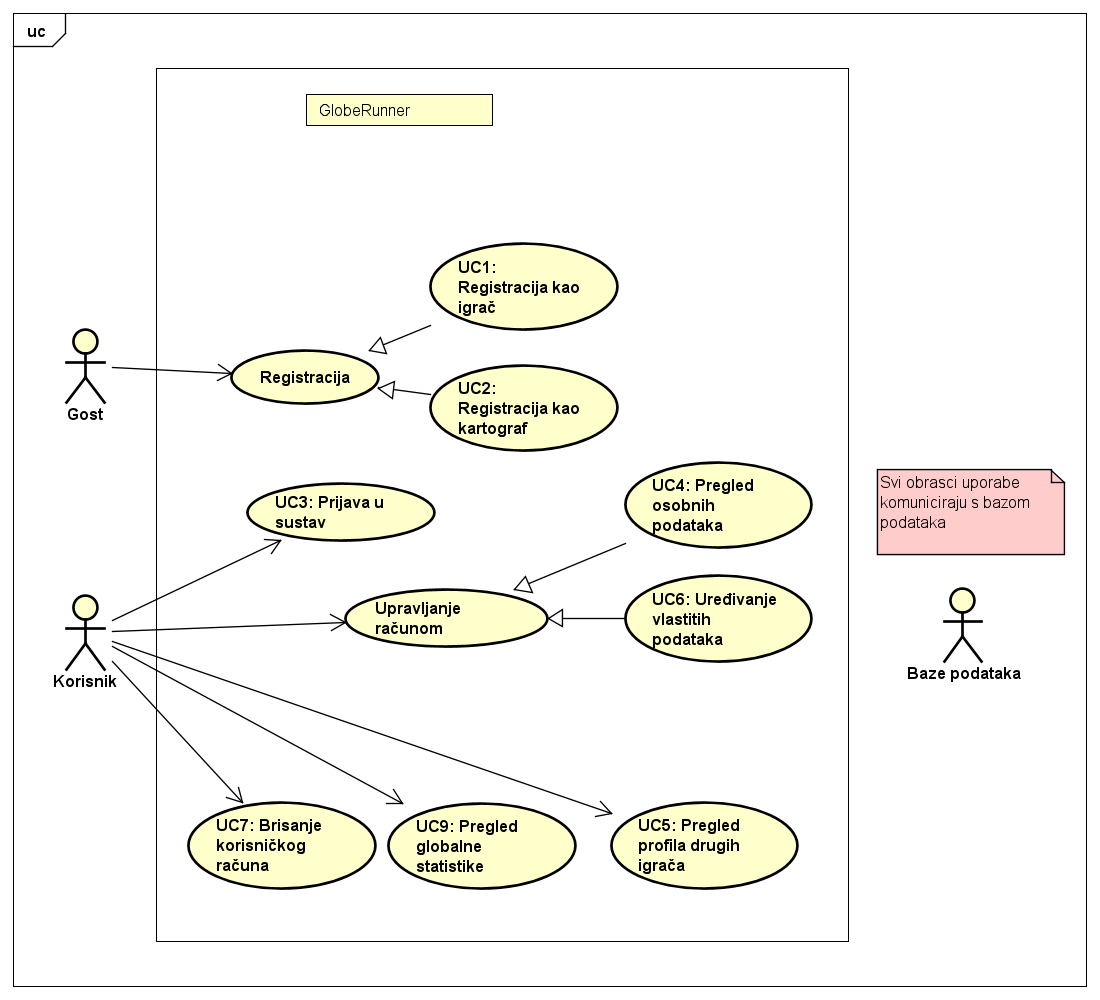
\includegraphics[scale=0.5]{slike/UCDiagrami/korisnik.png} %veličina slike u odnosu na originalnu datoteku i pozicija slike
        			\centering
        			\caption{Dijagram obrasca uporabe, funkcionalnost gosta i korisnika}
        			\label{fig:promjene}
        		\end{figure}
					
				\begin{figure}[H]
        			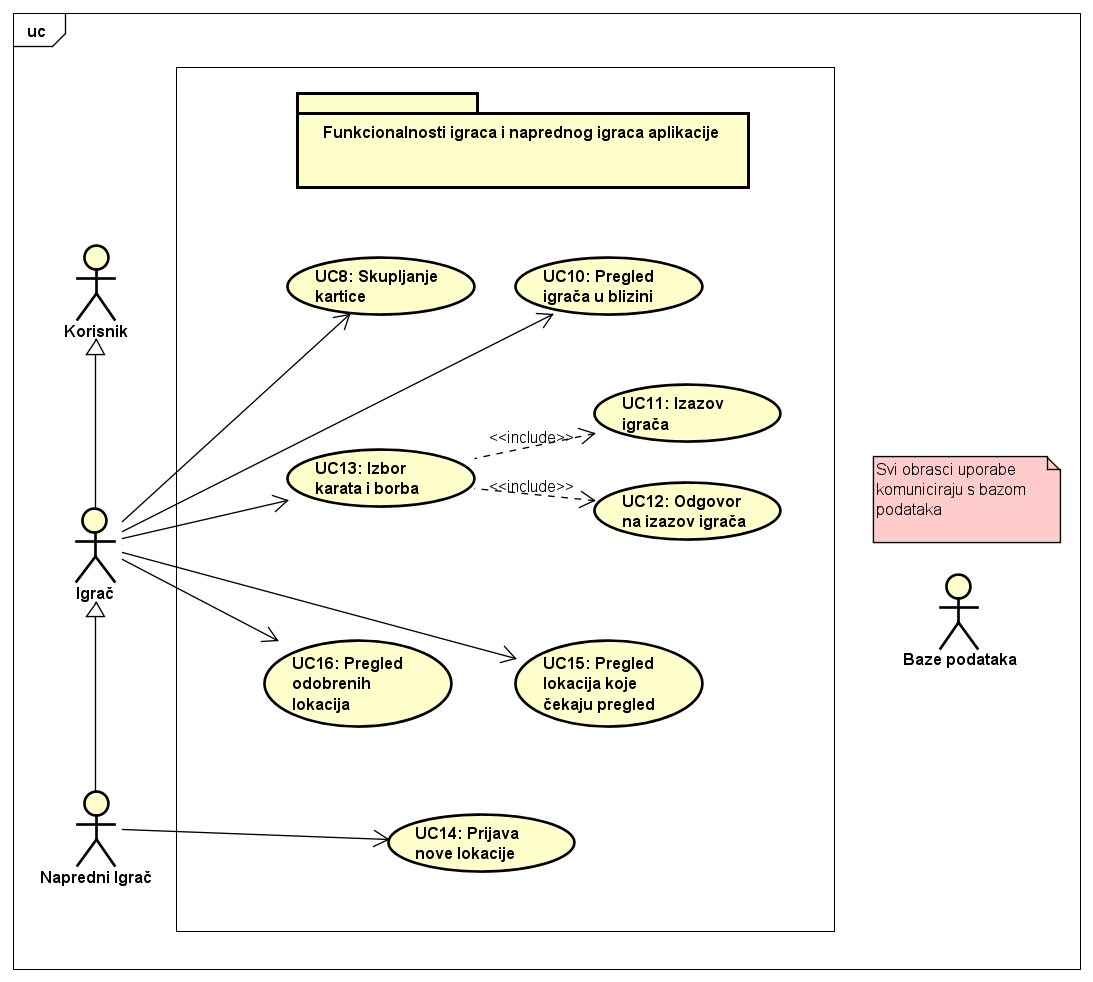
\includegraphics[scale=0.5]{slike/UCDiagrami/igrac.png} %veličina slike u odnosu na originalnu datoteku i pozicija slike
        			\centering
        			\caption{Dijagram obrasca uporabe, funkcionalnost igrača i naprednog igrača}
        			\label{fig:promjene}
        		\end{figure}
					
				\begin{figure}[H]
        			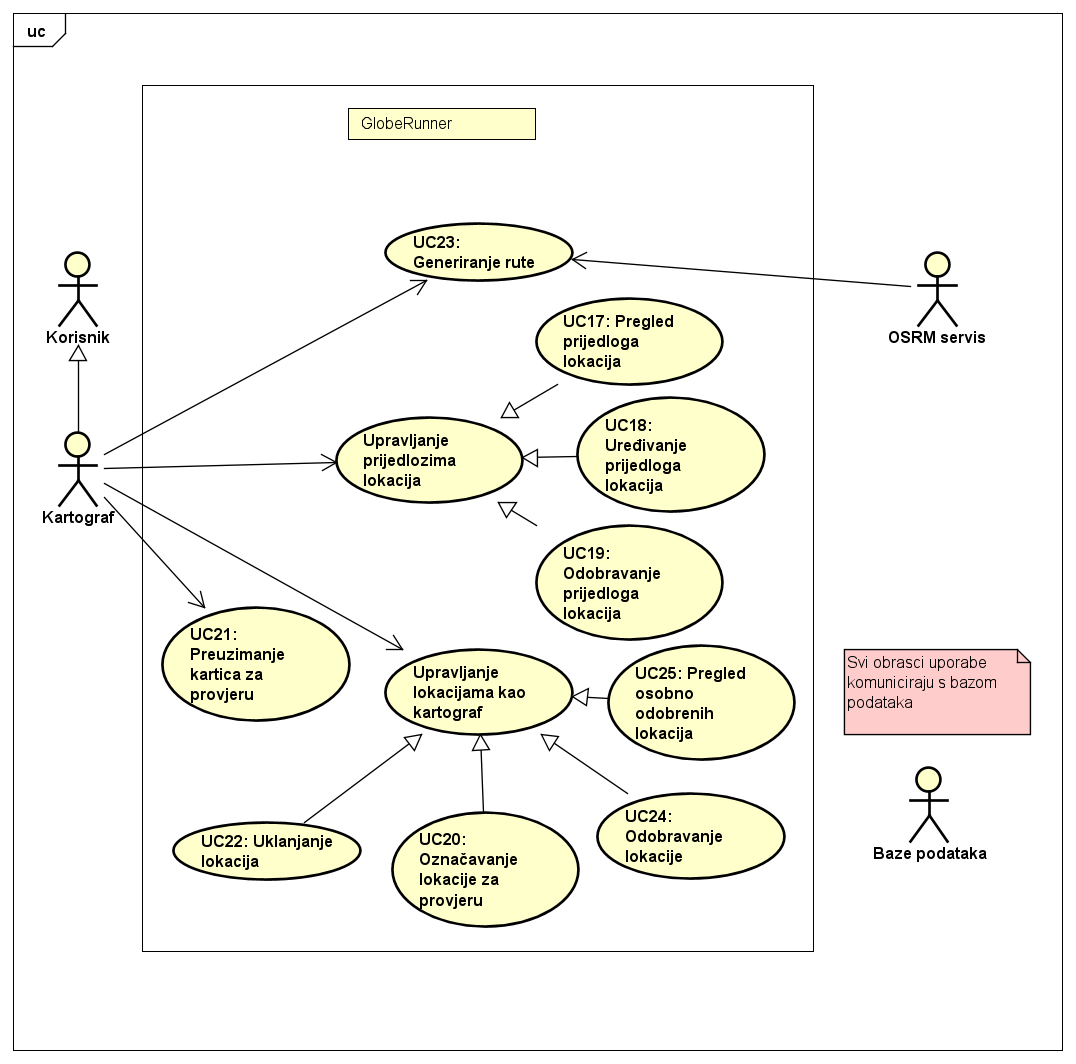
\includegraphics[scale=0.5]{slike/UCDiagrami/kartograf.png} %veličina slike u odnosu na originalnu datoteku i pozicija slike
        			\centering
        			\caption{Dijagram obrasca uporabe, funkcionalnost kartografa}
        			\label{fig:promjene}
        		\end{figure}
					
				\begin{figure}[H]
        			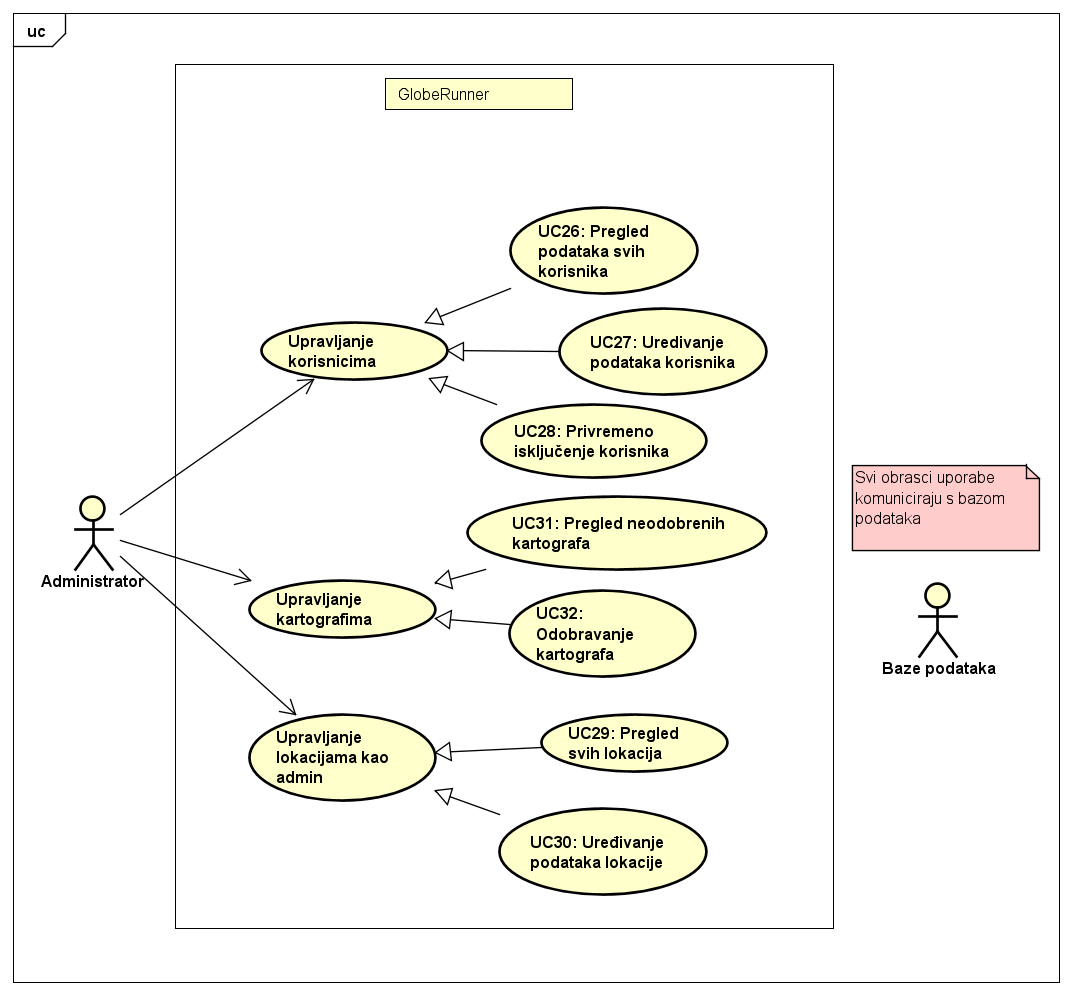
\includegraphics[scale=0.5]{slike/UCDiagrami/admin.png} %veličina slike u odnosu na originalnu datoteku i pozicija slike
        			\centering
        			\caption{Dijagram obrasca uporabe, funkcionalnost admina}
        			\label{fig:promjene}
        		\end{figure}
				
			\pagebreak
			\subsection{Sekvencijski dijagrami}
				
				\subsubsection{Obrazac uporabe UC14 - Prijava nove lokacije}
				
				Napredni igrač šalje zahtjev za dodavanje kartice te mu poslužitelj prikazuje sučelje za unos podataka o novoj kartici/lokaciji. Napredni igrač unosi sve podatke o kartici koju želi dodati te sprema provjere. Poslužitelj tada provjerava ispravnost unesenih podataka te ih, u slučaju uspješne validacije, sprema u bazu. Nakon toga, poslužitelj naprednom igraču ispisuje poruku o uspješnom dodavanju nove kartice/lokacije.
				
				\begin{figure}[H]
        			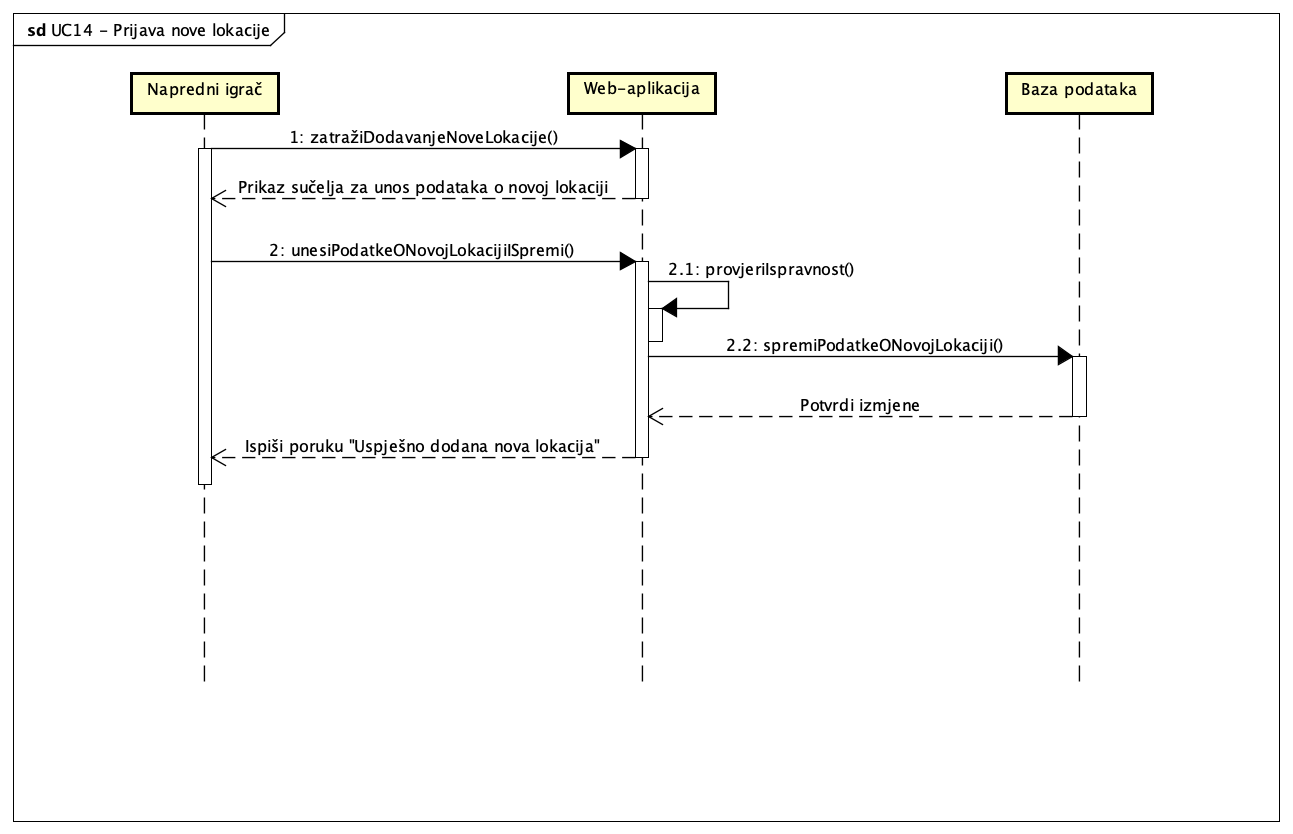
\includegraphics[scale=0.4]{slike/Sekvencijski dijagrami/UC14 - Prijava nove lokacije.png}
        			\centering
        			\caption{Sekvencijski dijagram za UC14}
        			\label{fig:promjene}
        		\end{figure}
				
				\pagebreak
				\subsubsection{Obrasci uporabe UC17 - Pregled prijedloga i UC18 - Uređivanje prijedloga}
				
				Kartograf šalje zahtjev za prikaz neodobrenih lokacija. Poslužitelj dohvaća neodobrene lokacije iz baze te ih prikazuje kartografu. Kartograf šalje zahtjev za izmjenu podataka o odabranoj lokaciji/kartici. Poslužitelj prikazuje kartografu sučelje za uređivanje postojećih podataka o neodobrenoj lokaciji. Kartograf unosi izmjene u prikazano sučelje. Ako kartograf pokuša zatvoriti prozor prije spremanja unesenih izmjena, poslužitelj ga upozorava da promjene nisu spremljene. Tada kartograf može odabrati svejedno zatvoriti prozor ili spremiti promjene. Ako odabere zatvoriti prozor prije spremanja, unesene izmjene neće biti spremljene u bazu. Ako odabere spremiti promjene, poslužitelj unesene podatke o lokaciji sprema u bazu te ispisuje poruku o uspješnoj izmjeni podataka.
				
				\begin{figure}[H]
        			\includegraphics[scale=0.3]{slike/Sekvencijski dijagrami/UC17 - Pregled prijedloga, UC18 - Uređivanje prijedloga.png}
        			\centering
        			\caption{Sekvencijski dijagram za UC17, UC18}
        			\label{fig:promjene}
        		\end{figure}
        		
        		\pagebreak
        		\subsubsection{Obrasci uporabe UC21 - Preuzimanje kartice za provjeru i UC23 - Generiranje rute}
        		
        		Kartograf šalje zahtjev za prikaz kartica koje trebaju terensku provjeru. Poslužitelj dohvaća kartice koje trebaju terensku provjeru iz baze te ih prikazuje kartografu. Kartograf šalje zahtjev za preuzimanjem kartice za provjeru. Poslužitelj u bazu podataka bilježi da je kartica preuzeta za provjeru te bilježi koji kartograf ju je preuzeo. Kartograf prije generiranja rute još jednom šalje zahtjev za prikaz neodobrenih lokacija. Poslužitelj ih dohvaća iz baze podataka te prikazuje kartografu. Kartograf šalje zahtjev za generiranje rute. Poslužitelj iz baze dohvaća kartice koje je taj kartograf preuzeo za provjeru te ih šalje OSRM servisu i zahtjeva generiranje rute. OSRM servis poslužitelju vraća generiranu rutu, a poslužitelj ju prikazuje kartografu.
				
				\begin{figure}[H]
        			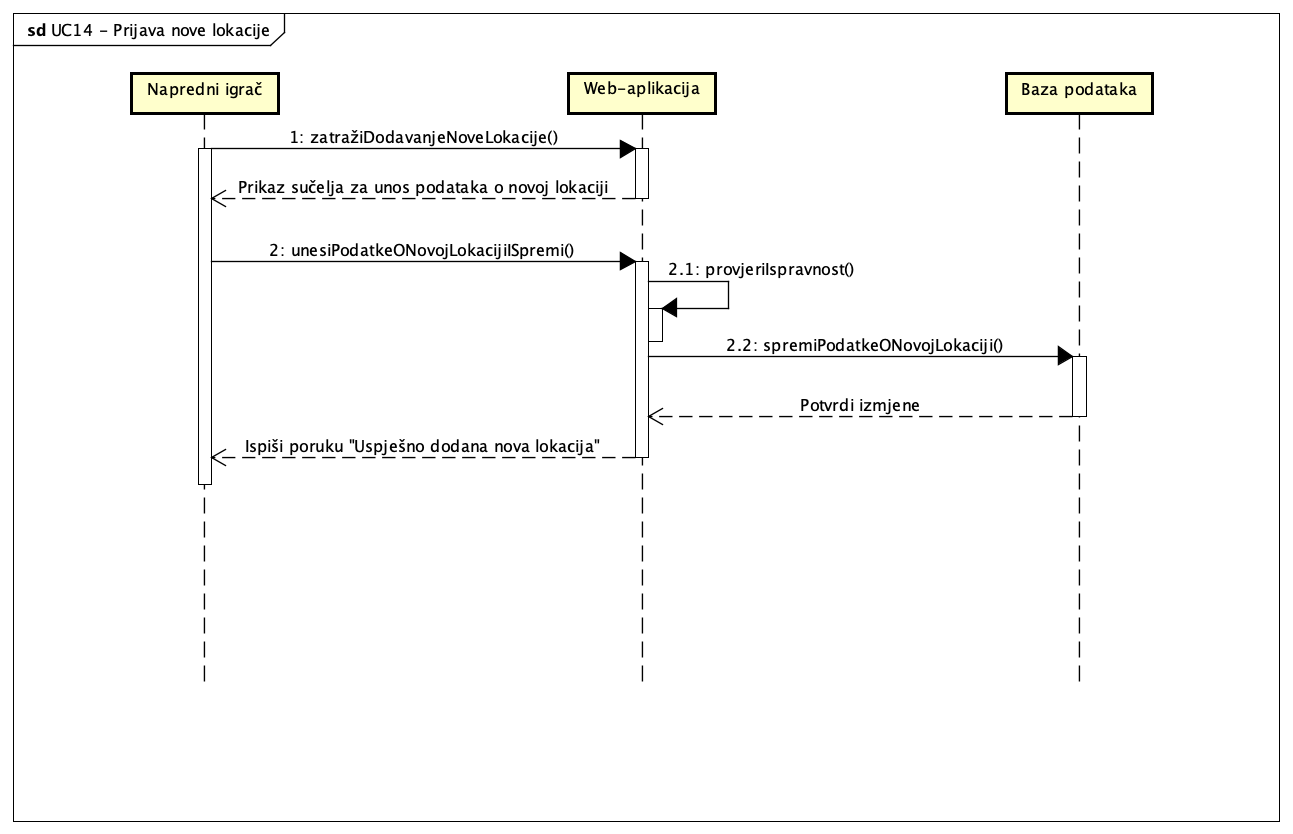
\includegraphics[scale=0.4]{slike/Sekvencijski dijagrami/UC14 - Prijava nove lokacije.png}
        			\centering
        			\caption{Sekvencijski dijagram za UC21, UC23}
        			\label{fig:promjene}
        		\end{figure}
	    \pagebreak
		\section{Ostali zahtjevi}
		\begin{packed_item}
		    \item Sustav treba omogućiti rad više korisnika u stvarnom vremenu
			\item Korisničko sučelje i sustav moraju podržavati hrvatsku abecedu (dijakritičke znakove) pri unosu i prikazu tekstualnog sadržaja
			\item Izvršavanje dijela programa u kojem se pristupa bazi podataka ne smije trajati duže od nekoliko sekundi
			\item Sustav treba biti implementiran kao web aplikacija koristeći objektno-orijentirane jezike
			\item Neispravno korištenje korisničkog sučelja ne smije narušiti funkcionalnost i rad sustava
			\item Sustav treba biti jednostavan za korištenje, korisnici se moraju znati koristiti sučeljem bez opširnih uputa
			\item Nadogradnja sustava ne smije narušavati postojeće funkcionalnosti sustava
			\item Sustav kao valutu koristi EURO
			\item Veza s bazom podataka mora biti kvalitetno zaštićena, brza i otporna na vanjske greške
			\item Pristup sustavu mora biti omogućen iz javne mreže pomoću HTTPS
			\item Rukovanje osobnim podatcima treba biti usklađeno s važećim direktivama
			\item Sustav treba koristiti GPS za pozicioniranje igrača i kartica na karti
			\item Sustav treba koristiti OSRM servis za rješavanje problema trgovačkog putnika
			
		\end{packed_item}